\documentclass[letterpaper,12pt]{article}
\usepackage[margin=64pt]{geometry}
\usepackage{amsthm}
\usepackage{amsmath}
\usepackage{amssymb}
\usepackage{parskip}
\usepackage{graphicx}
\usepackage{enumerate}
\usepackage{hyperref}
\usepackage{listings}
\newcommand{\transpose}{^{\mbox{\tiny T}}}


\begin{document}
\thispagestyle{empty}

\hrule \vspace{0.5em}
\noindent {\bf CFRM 462: Introduction to Computational Finance and Econometrics} \hfill Homework 4 \newline \hrule

\vspace{1em}

\enumerate
\item \begin{lstlisting}
w = 100000

VBLTX = quantile(lab4Returns.z[,1],c(0.01,0.05))
FMAGX = quantile(lab4Returns.z[,2],c(0.01,0.05))
SBUX = quantile(lab4Returns.z[,3],c(0.01,0.05))

p_var = c(VBLTX,FMAGX,SBUX)*w
    1%     5%     1%     5%     1%     5% 
 -7598  -4054 -22434  -9327 -39014 -14459 
\end{lstlisting}
Starbucks has the highest 1\% VaR and the highest 5\% VaR, whereas the Vanguard Long Term Bond Fund has the lowest VaR. This is not surprising considering the bond fund is diversified and does not have a high correlation with the S\&P (low beta).

\item The pair FMAGX and SBUX have the highest correlation around 0.44, everything else is weakly correlated $\approx$[+6,-6]\% \\ 
	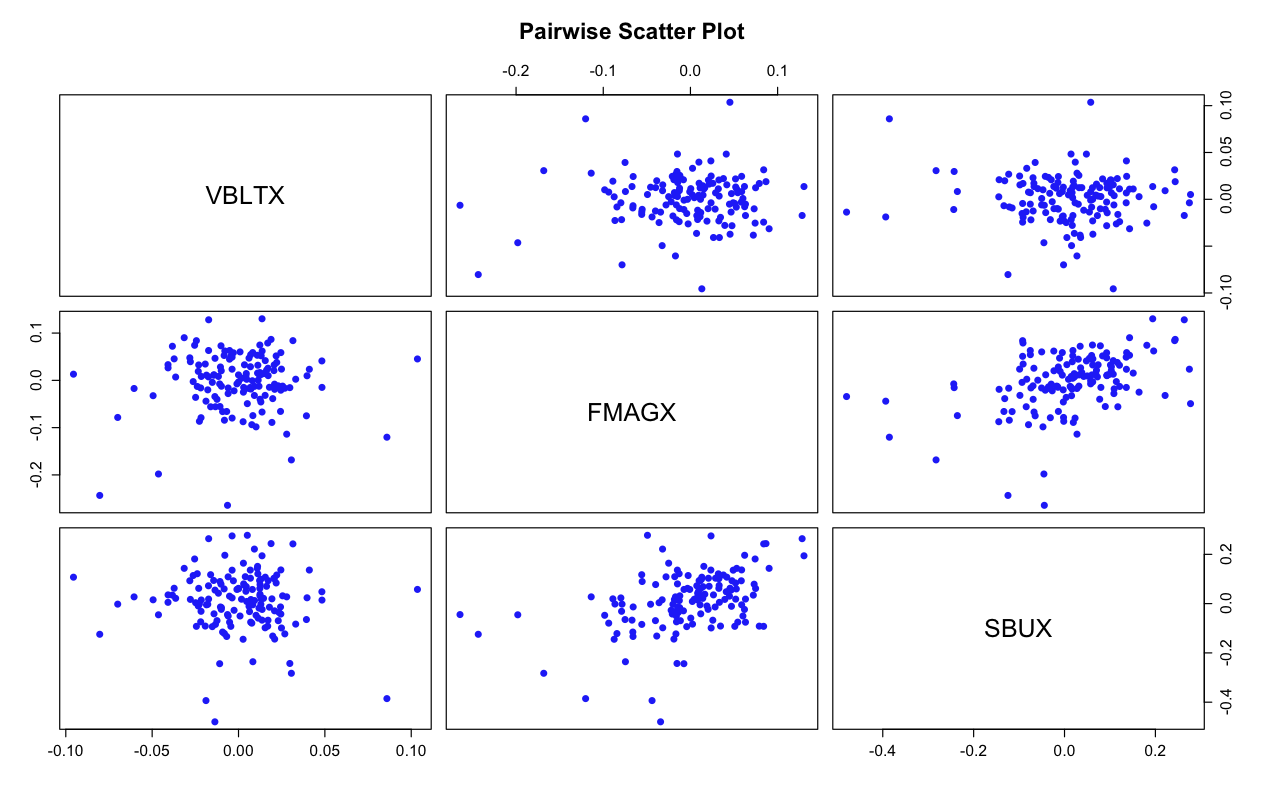
\includegraphics[scale = 0.35]{Pairs} \\

\item  Plots \\
    \includegraphics[scale = 0.5]{corrplot} \\
    \includegraphics[scale = 0.5]{corrplot_mixed}

\item The variance of SBUX is the largest with the covariance of SBUX, FMAGX the second largest. The lowest covariance is between VBLTX and SBUX. The assets with the highest positive correlation were FMAGX, and SBUX, while the lowest was between VBLTX and SBUX.
\begin{lstlisting}
    > cov(lab4Returns.z)
              VBLTX   FMAGX      SBUX
    VBLTX  0.000680 0.00011 -0.000186
    FMAGX  0.000110 0.00371  0.003187
    SBUX  -0.000186 0.00319  0.014261
    > 
    > #Same as cov matrix 
    > var(lab4Returns.z)
              VBLTX   FMAGX      SBUX
    VBLTX  0.000680 0.00011 -0.000186
    FMAGX  0.000110 0.00371  0.003187
    SBUX  -0.000186 0.00319  0.014261
    > 
    > #Sample Correlation Matrix
    > cor(lab4Returns.z)
            VBLTX  FMAGX    SBUX
    VBLTX  1.0000 0.0691 -0.0597
    FMAGX  0.0691 1.0000  0.4381
    SBUX  -0.0597 0.4381  1.0000
\end{lstlisting}

\item \hspace{18em} ACF \\
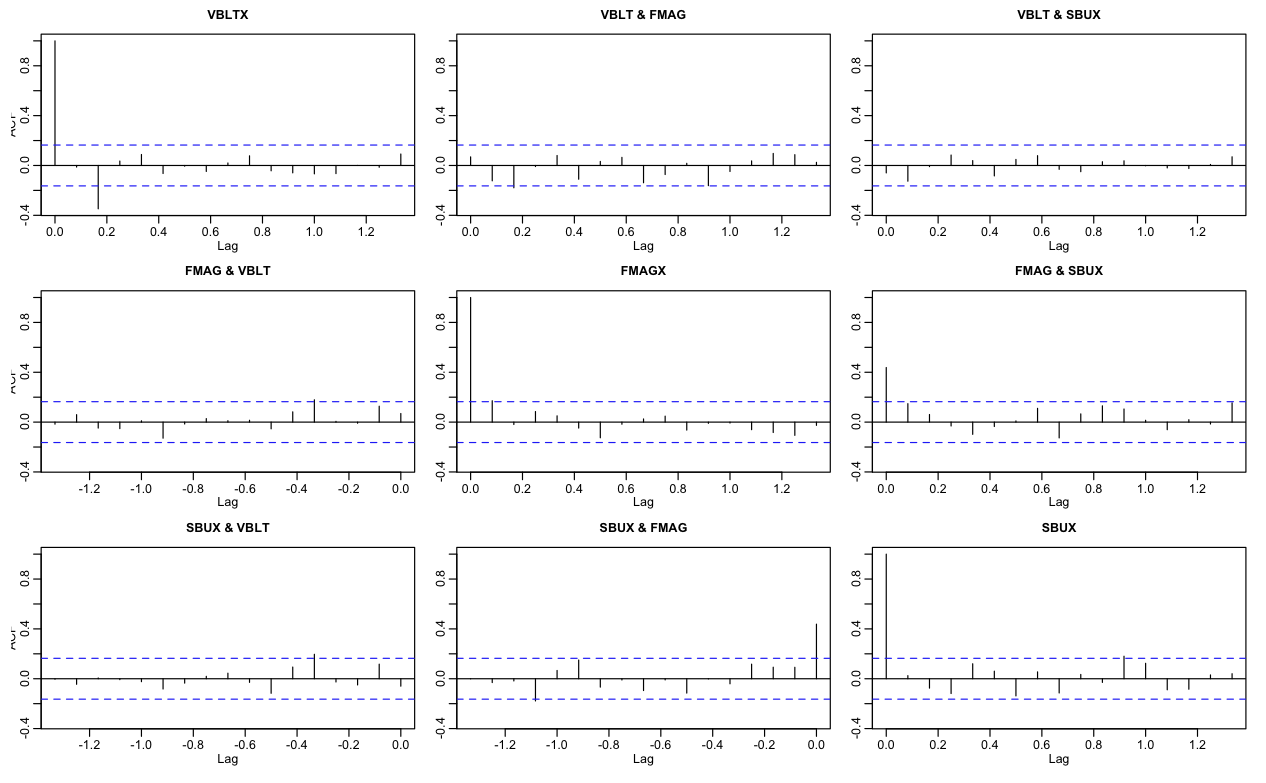
\includegraphics[scale = 0.35]{acf}

\item SBUX has the highest expected value but also the highest variance, whereas FMAGX has the lowest expected return and VBLTX has the lowest variance. 
\begin{lstlisting}
      muhat.vals sigma2hat.vals sigmahat.vals covhat.vals rhohat.vals
VBLTX   0.000429        0.00068        0.0261    0.000110      0.0691
FMAGX  -0.002770        0.00371        0.0609   -0.000186     -0.0597
SBUX    0.011394        0.01426        0.1194    0.003187      0.4381
\end{lstlisting}

\item The expected return for VBLTX has the least bias, whereas SBUX has the highest. The same goes for the variance, and sd. Interestingly, the precision of rho between these assets is the lowest, even though they exhibit drastically different characteristics.
\begin{lstlisting}
    > se.mu
      VBLTX   FMAGX    SBUX 
    0.00218 0.00509 0.00999 
    > se.sigma2
       VBLTX    FMAGX     SBUX 
    8.05e-05 4.39e-04 1.69e-03 
    > se.sigma
      VBLTX   FMAGX    SBUX 
    0.00154 0.00360 0.00706 
    > se.rho
    VBLTX,FMAGX  VBLTX,SBUX  FMAGX,SBUX 
        0.00578    -0.00499     0.03664 
\end{lstlisting}

\item The confidence interval for SBUX is the largest due to the large standard error and the lowest for VBLTX due to the low SE.

\begin{lstlisting}
> mu.95
      mu.lower mu.upper
VBLTX -0.00393  0.00479
FMAGX -0.01296  0.00742
SBUX  -0.00858  0.03137
> mu.99
      mu.lower2 mu.upper2
VBLTX  -0.00612   0.00697
FMAGX  -0.01805   0.01251
SBUX   -0.01857   0.04135
> var.95
      var.lower var.upper
VBLTX   0.00052  0.000841
FMAGX   0.00283  0.004587
SBUX    0.01089  0.017635
> var.99
      var.lower2 var.upper2
VBLTX   0.000439   0.000922
FMAGX   0.002393   0.005025
SBUX    0.009202   0.019321
> sd.95
      sd.lower sd.upper
VBLTX   0.0230   0.0292
FMAGX   0.0537   0.0681
SBUX    0.1053   0.1335
> sd.99
      sd.lower2 sd.upper2
VBLTX    0.0215    0.0307
FMAGX    0.0501    0.0717
SBUX     0.0982    0.1406
> rho.95
            rho.lower rho.upper
VBLTX,FMAGX    0.0576    0.0807
VBLTX,SBUX    -0.0497   -0.0697
FMAGX,SBUX     0.3649    0.5114
> rho.99
            rho.lower2 rho.upper2
VBLTX,FMAGX     0.0518     0.0865
VBLTX,SBUX     -0.0447    -0.0747
FMAGX,SBUX      0.3282     0.5481
\end{lstlisting}

\item \begin{lstlisting}
#Var = mu + sigma * qnorm(p)
obs_var.05 = mu_hat + sigma_hat * qnorm(0.05)
obs_var.01 = mu_hat + sigma_hat * qnorm(0.01)

#Convert to simple return
obs_var.95 = (exp(obs_var.05)-1)*w
obs_var.99 = (exp(obs_var.01)-1)*w

obs_var.95
obs_var.99
\end{lstlisting}
\vfill \hrule \vspace{2mm} \centerline {\tt \tiny http://computational-finance.uw.edu}
\end{document}